\newpage
\section{}

\subsection{Examine the Ni-Al-Ta ternary phase diagram, is there a strong temperature dependence?}

To evaluate if there is a strong dependence on temperature, the Ni-Al-Ta ternary phase diagram was generated using the \textit{phase diagram} tool at different temperatures, from $800^{\circ}$C to $1300^{\circ}$C, the resulting diagrams are shown in figure \ref{fig:diagram02}.

Figures \ref{fig:800C} and \ref{fig:900C} present the ternary phase diagram for the alloy at $800$°C and $900$°C respectively, from the diagrams it can be seen a small increase in the $\gamma$ phase  region. This can be noted in the $\gamma$ boundary line that moves from a mole percent of $12\%$ in figure \ref{fig:800C}, to approximately $14\%$ in the Al axis in figure \ref{fig:900C}.

\begin{figure}[h]
  \centering
  \subfloat[800°C\label{fig:800C}]{
    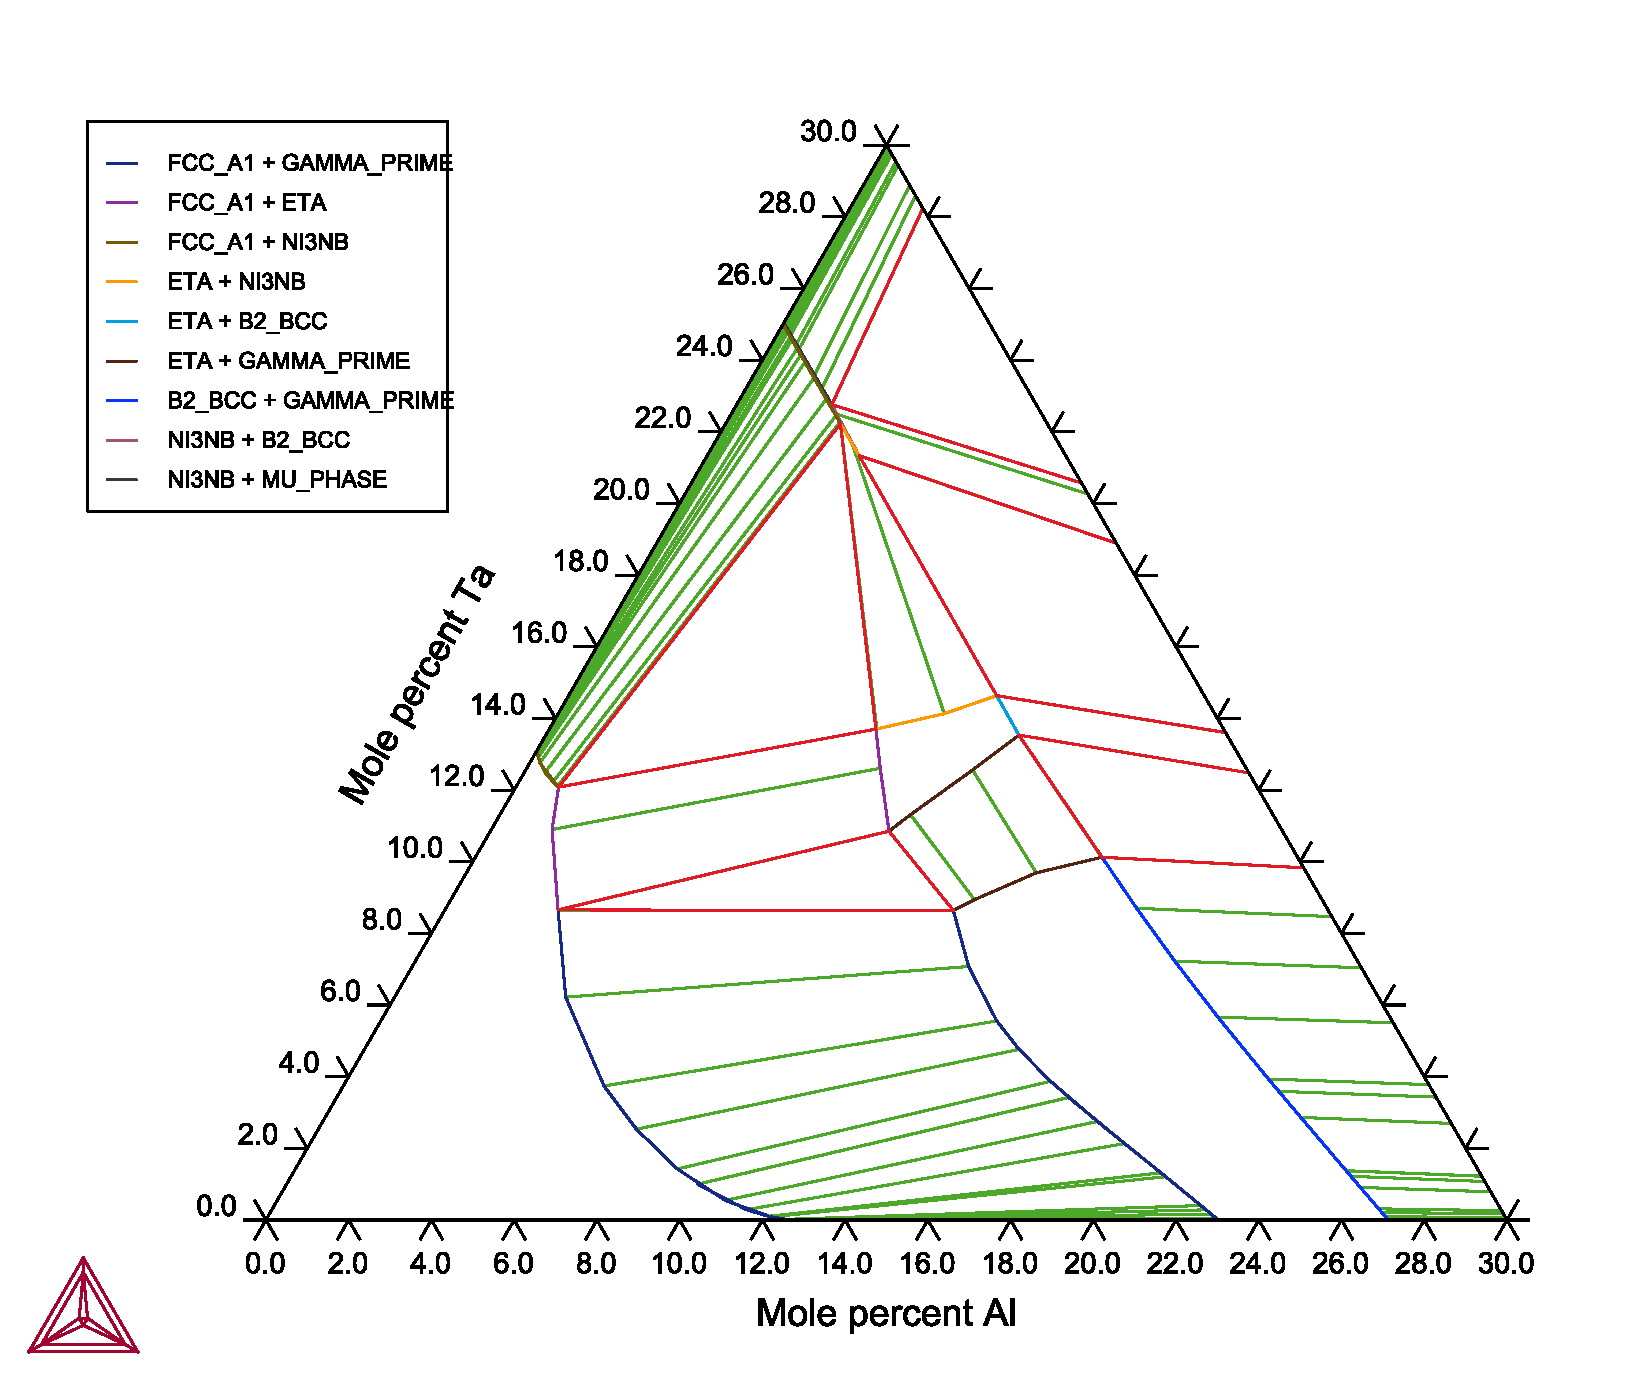
\includegraphics[width=0.5\textwidth]{graficas/Q2_NiAlTa_ternary_800C.pdf}
    }
  \subfloat[900°C\label{fig:900C}]{
    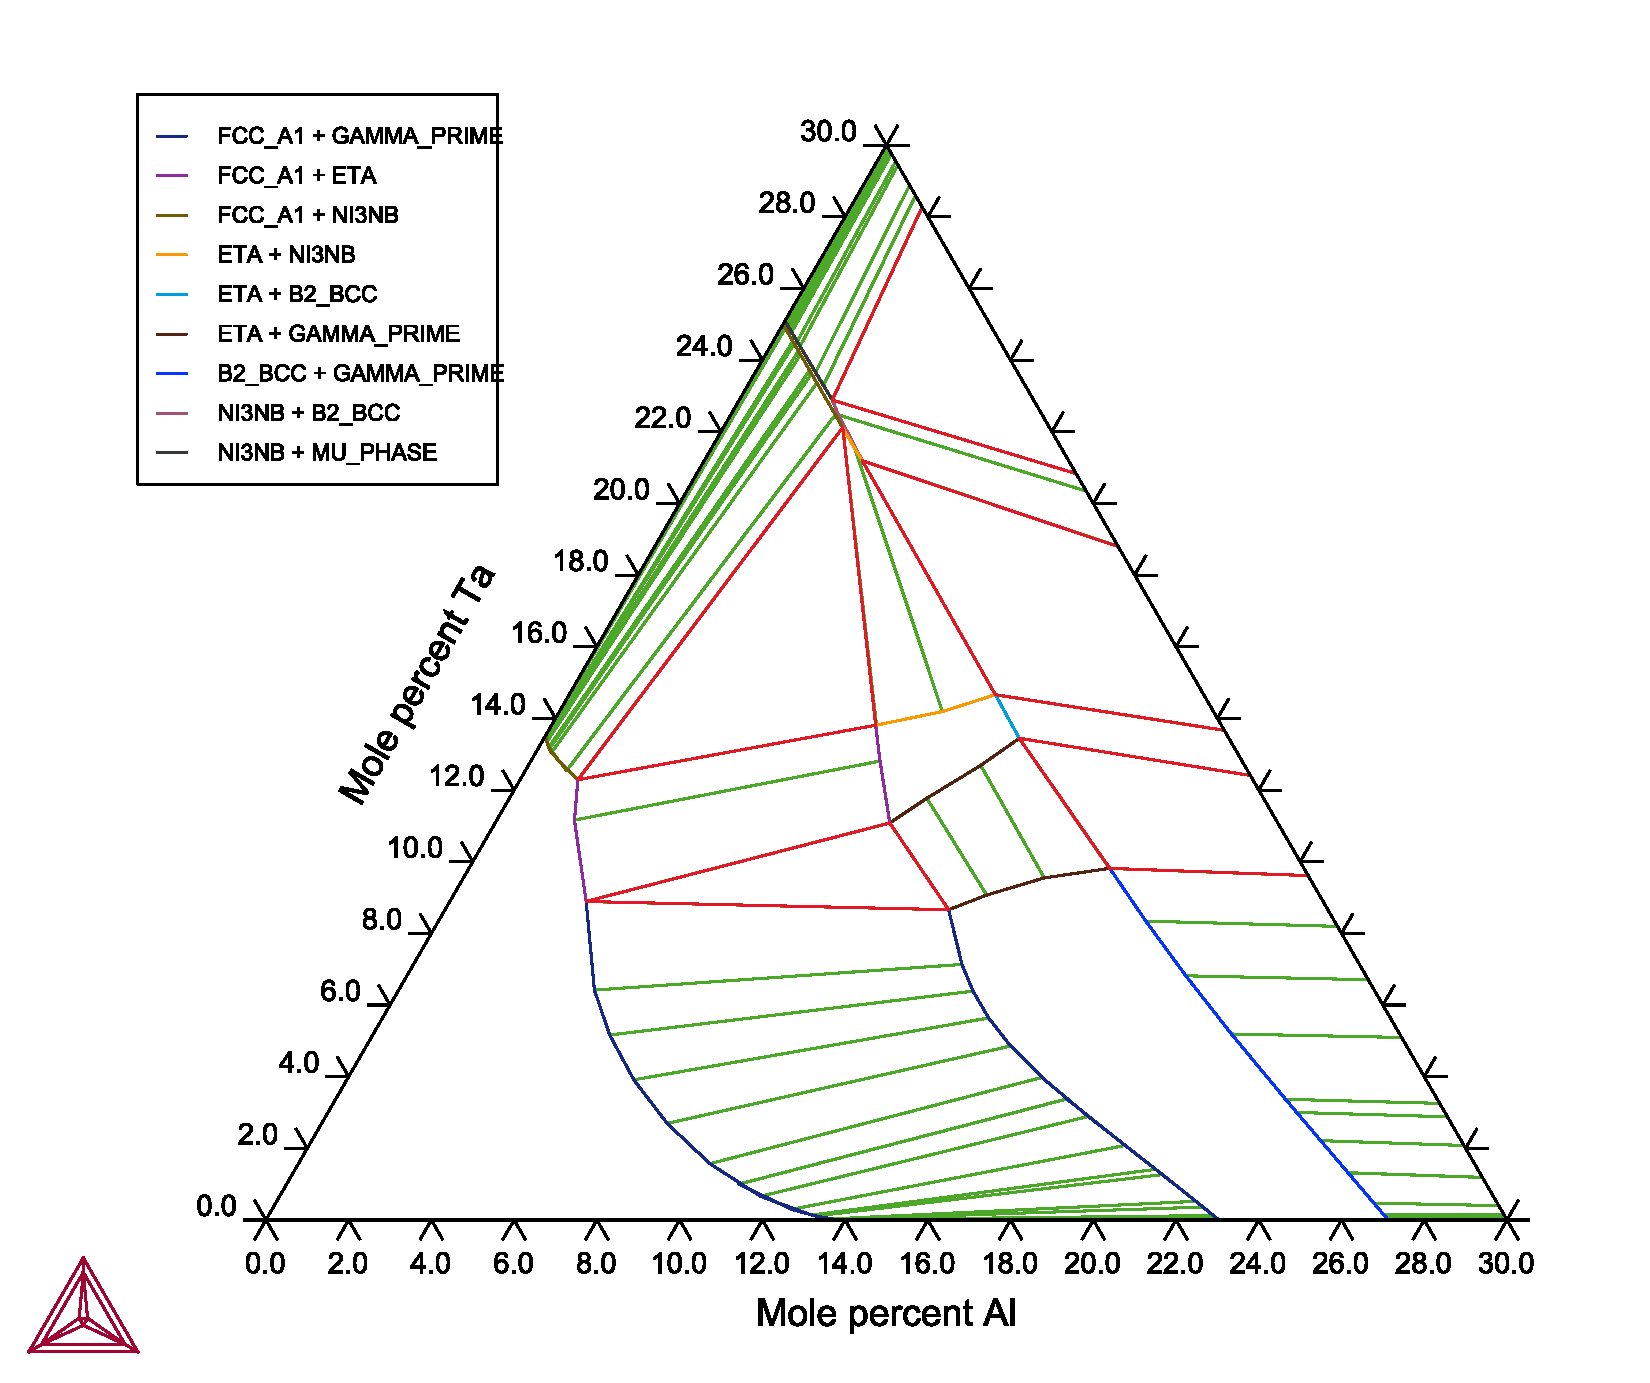
\includegraphics[width=0.5\textwidth]{graficas/Q2_NiAlTa_ternary_900C.pdf}
    }
  \caption{\centering Ni-Al-Ta ternary diagram at different temperatures \\
  \textit{Sourcce: diagrams generated with ThermoCalc \citep{thermocalc}}}
  \label{fig:diagram02}
\end{figure}

As temperature increases, the increase on the $\gamma$ phase is more evident, where the bondary line of the $\gamma$ phase moves from approximately $15\%$ at $10000$°C, in figure \ref{fig:1000C}, to $16\%$ at $1100$°C, in figure \ref{fig:1100C}. The change is more evident as the temperature increases to $1200$°C and $1300$°C, as it is shown in figures \ref{fig:1200C} and \ref{fig:1300C}; where at a temperature of $1200$°C the boundary can be found at $18\%$ and when the temperature is increased to $1300$°C the boundary is at $20\%$.

\begin{figure}[H]
  \centering
  \ContinuedFloat
  \subfloat[1000°C\label{fig:1000C}]{
    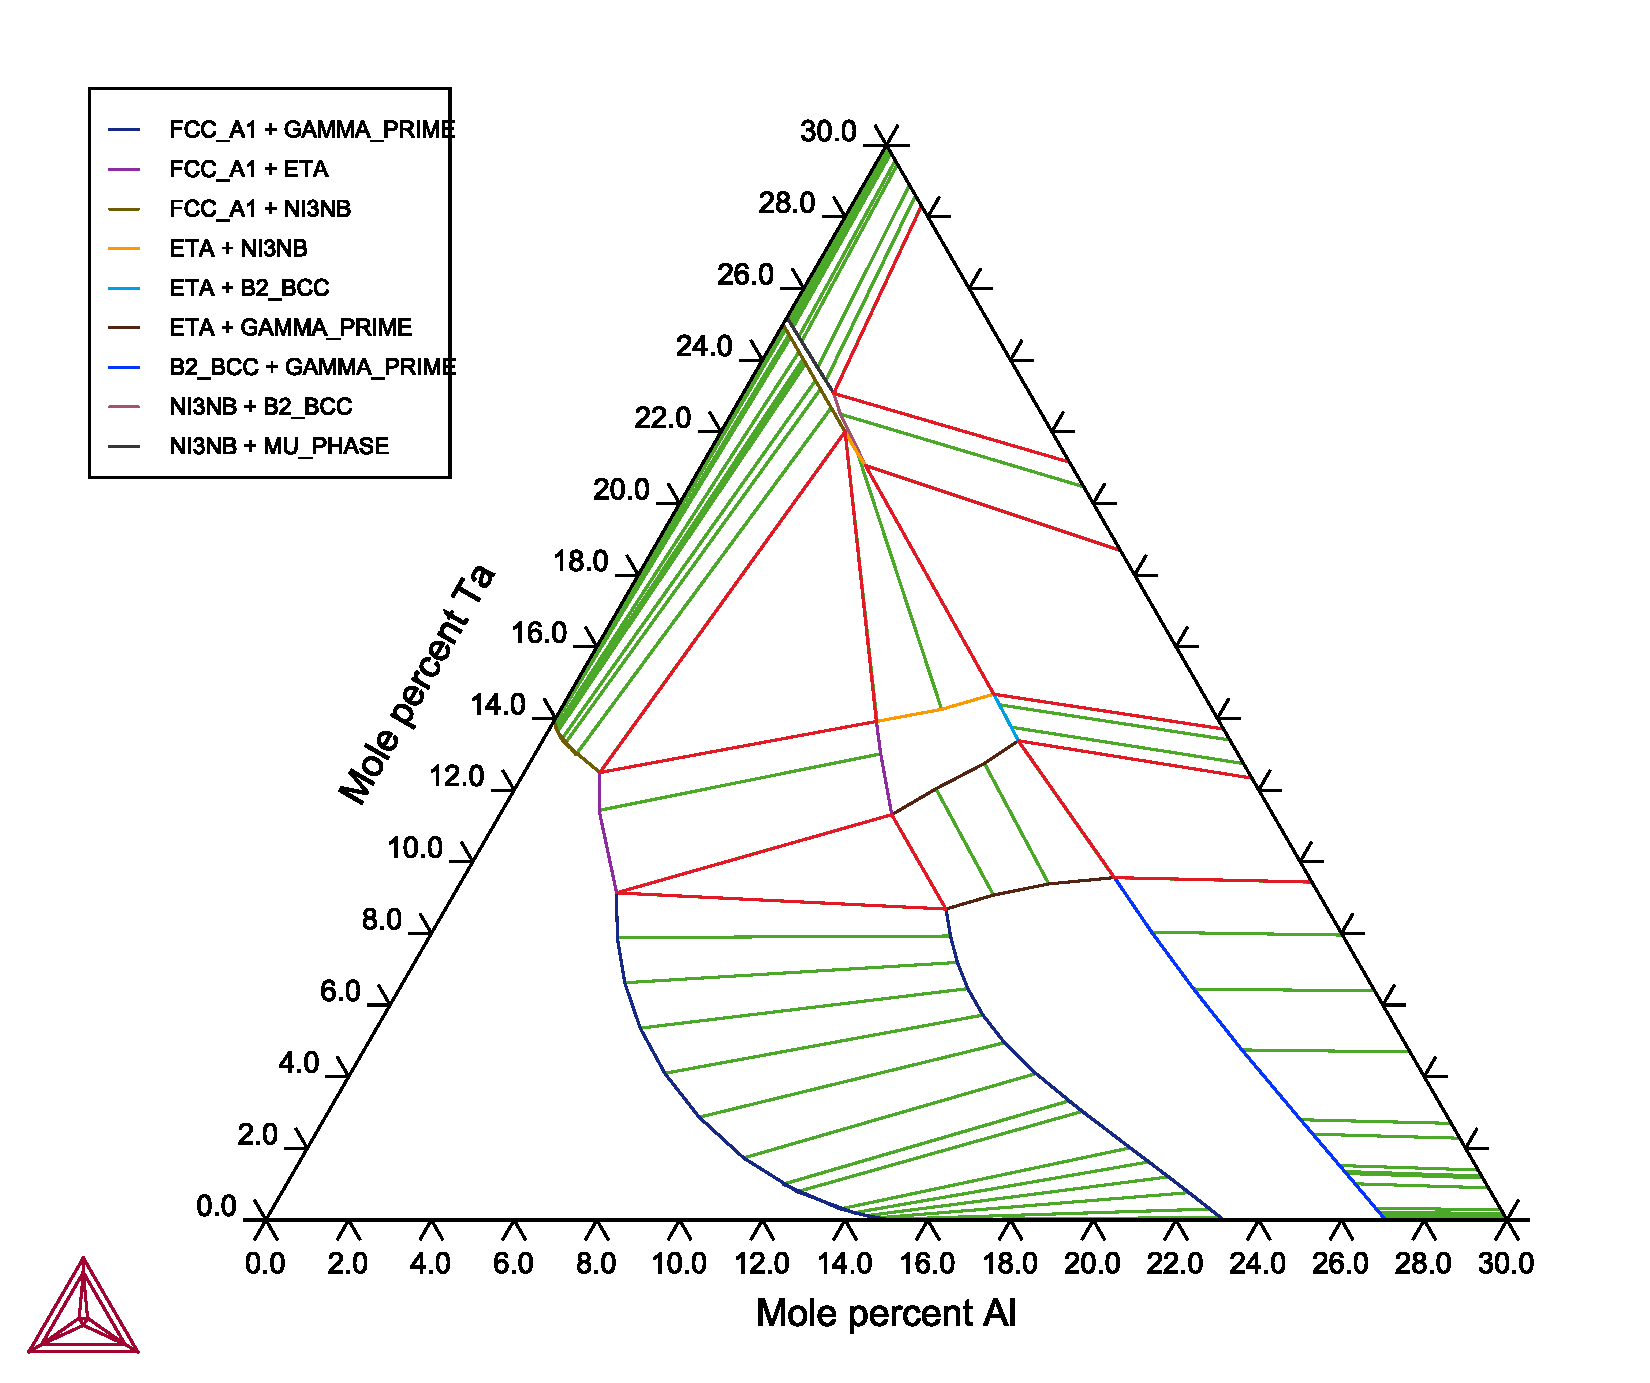
\includegraphics[width=0.5\textwidth]{graficas/Q2_NiAlTa_ternary_1000C.pdf}
    }
  \subfloat[1100°C\label{fig:1100C}]{
    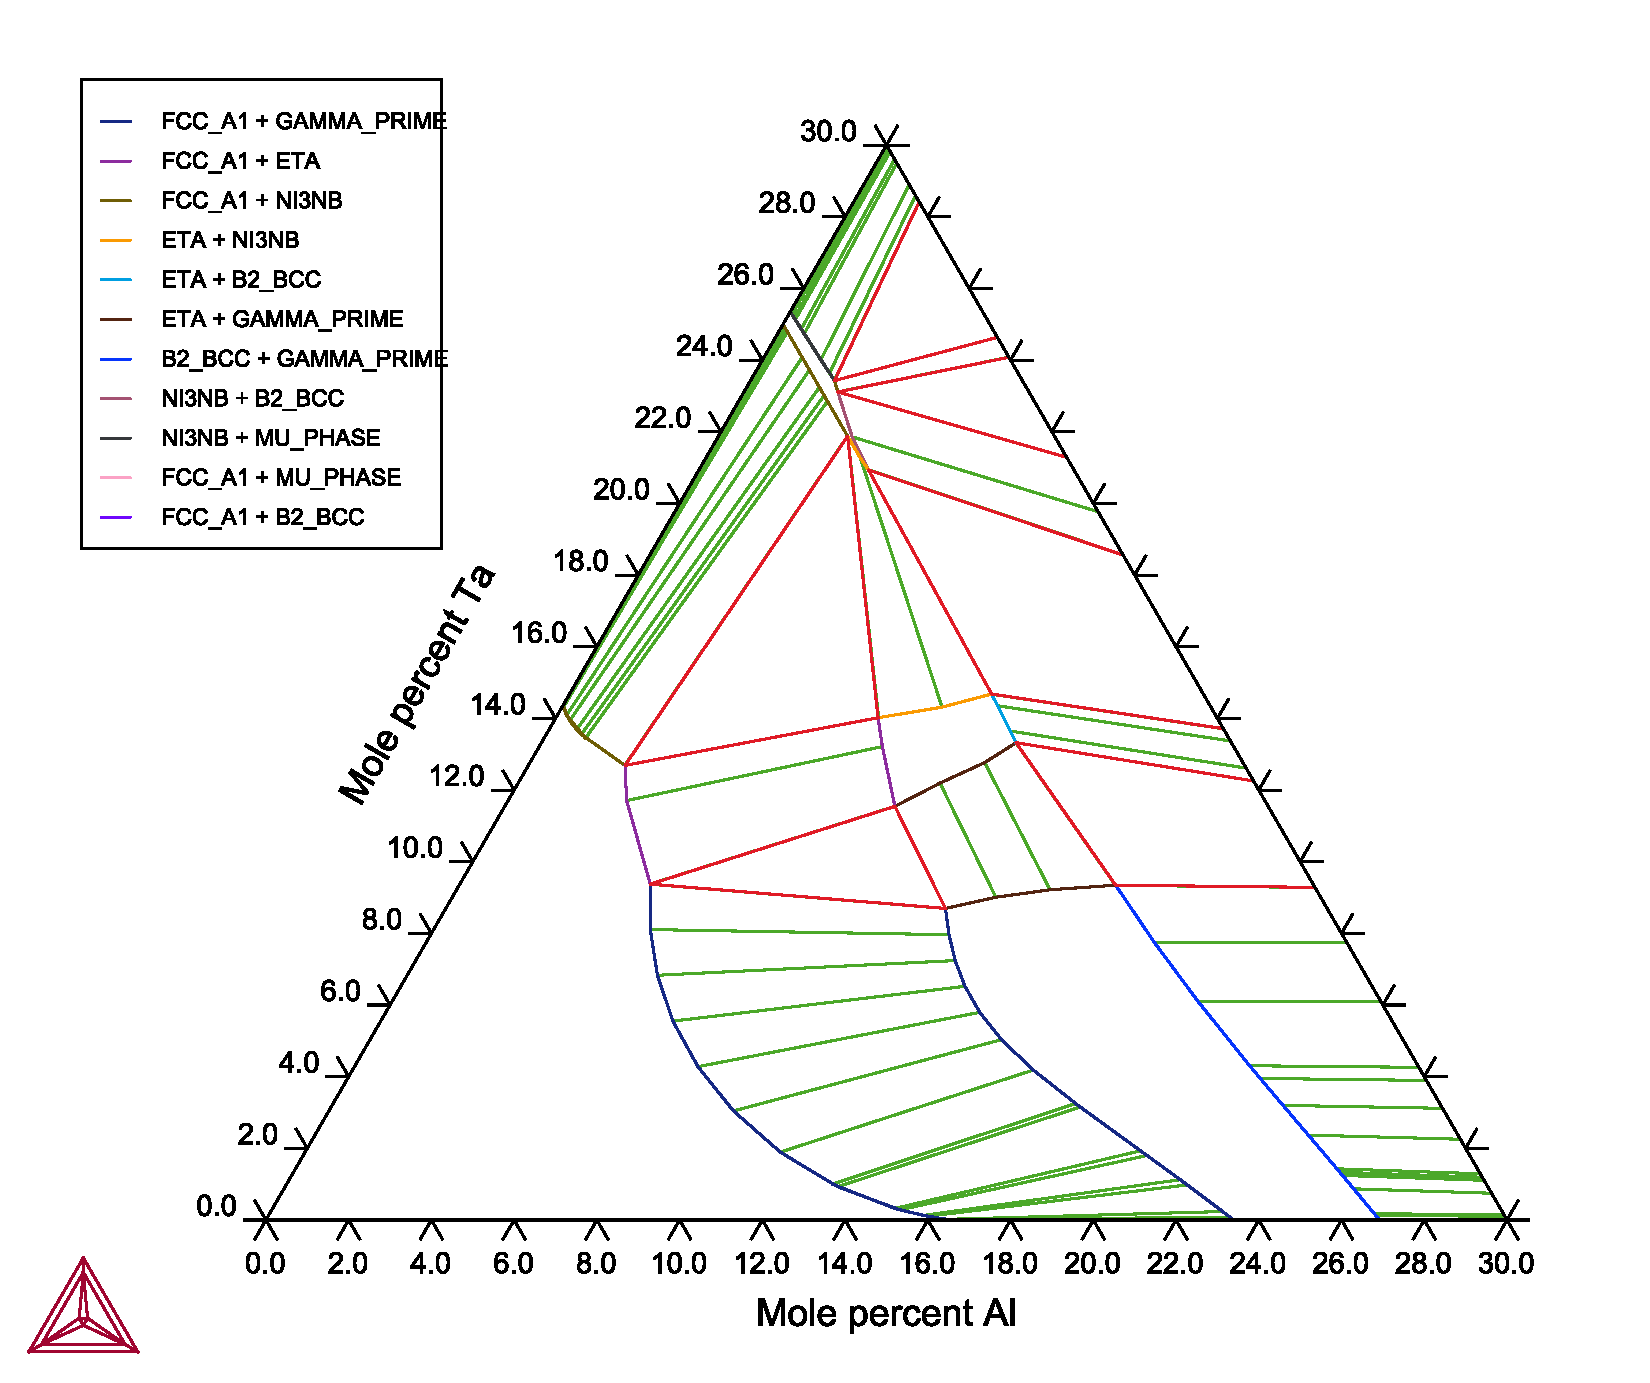
\includegraphics[width=0.5\textwidth]{graficas/Q2_NiAlTa_ternary_1100C.pdf}
    } \\
  \subfloat[1200°C\label{fig:1200C}]{
    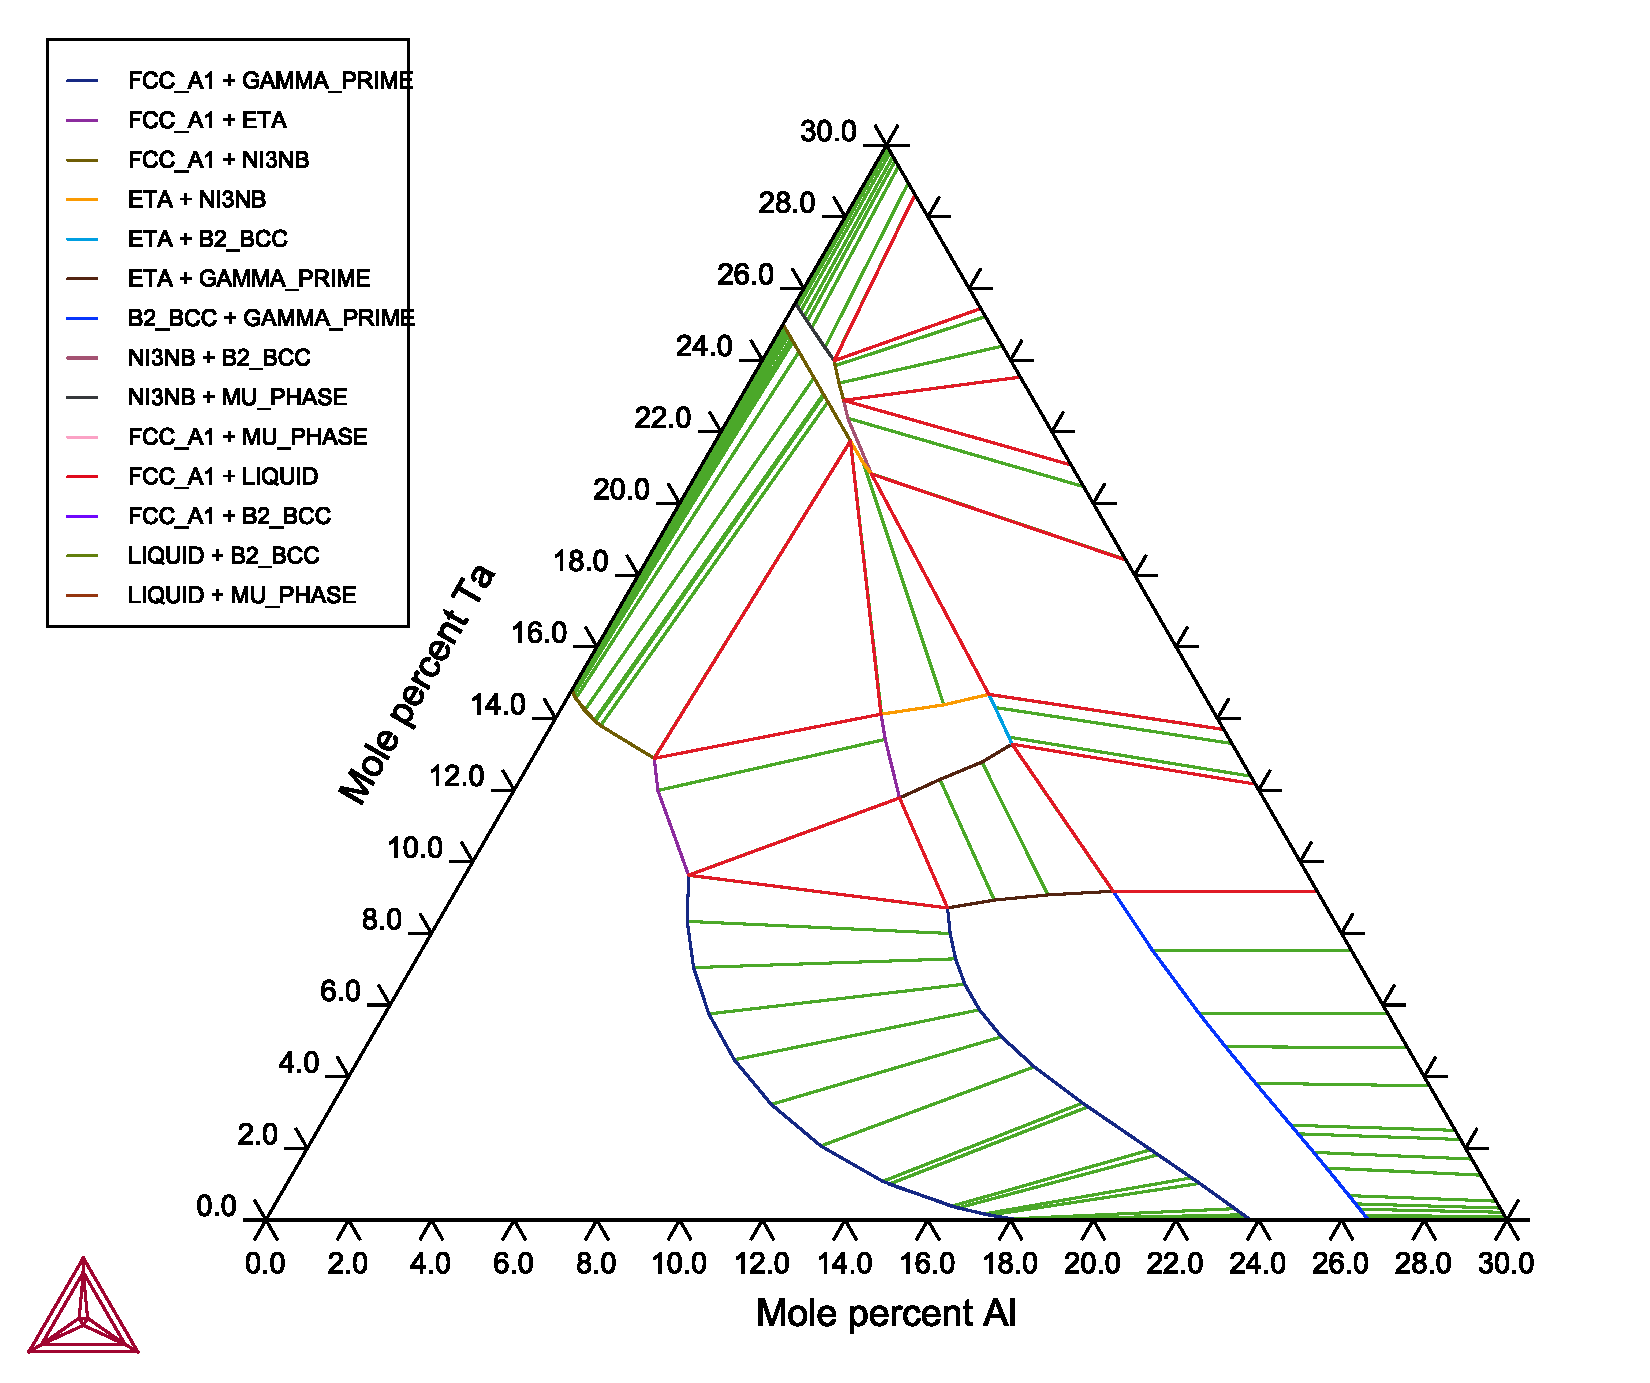
\includegraphics[width=0.5\textwidth]{graficas/Q2_NiAlTa_ternary_1200C.pdf}
    }
  \subfloat[1300°C\label{fig:1300C}]{
    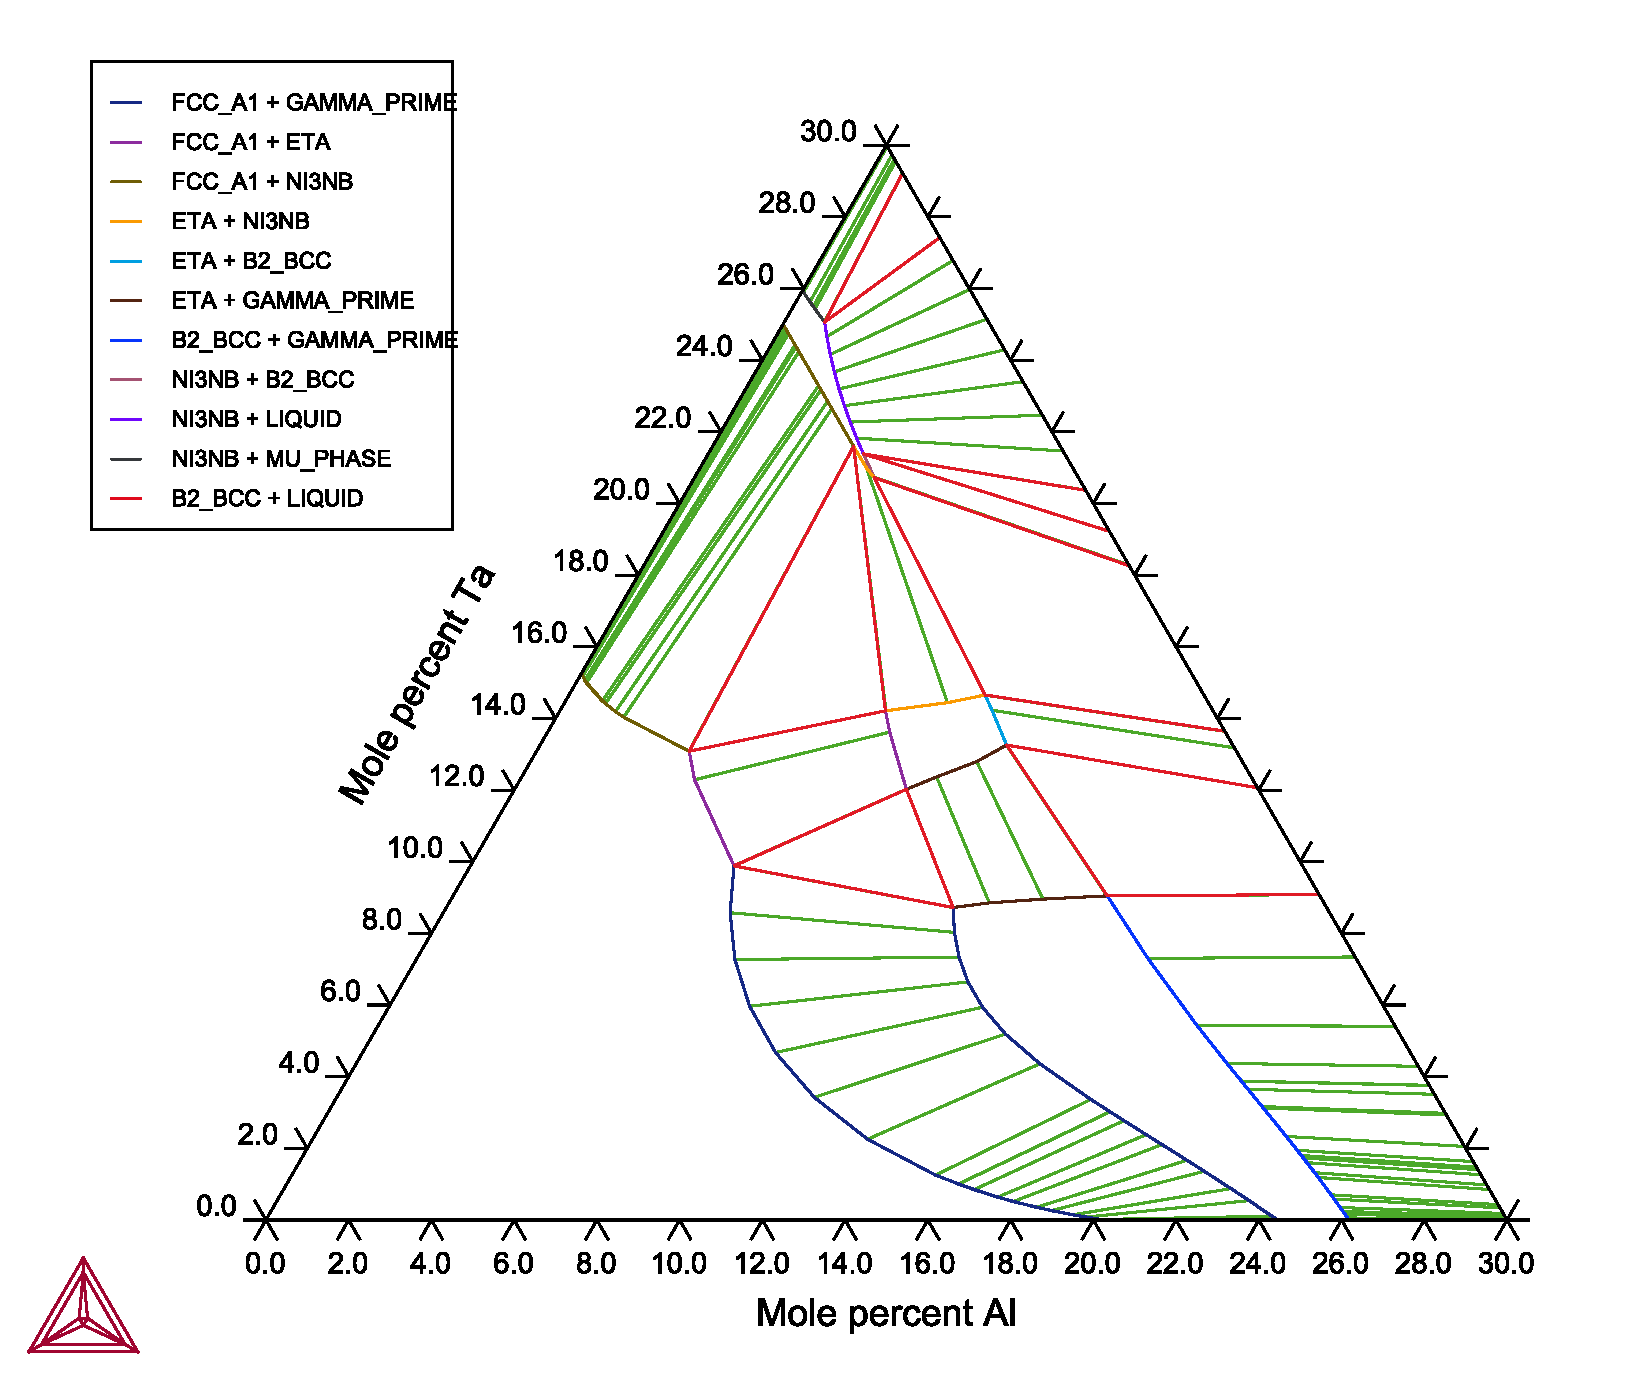
\includegraphics[width=0.5\textwidth]{graficas/Q2_NiAlTa_ternary_1300C.pdf}
    }
  \caption[]{\centering Ni-Al-Ta ternary diagram at different temperatures generated with \textit{ThermoCalc} \citep{thermocalc} (continued)}
\end{figure}

Along with the increase of the area that is ocuppied by the $\gamma$ phase, there is also a decrease on the area of the $\gamma'$ phase. These changes can indicate that there is a dependence on temperature on the equilibrium of the $\gamma$ and $\gamma'$ phases in the Ni-Al-Ta alloy.


\newpage
\subsection{Ni-Al-Ta alloys for which $\gamma'$ phase fraction is optimal}

The optimal fraction is that for which $\gamma'$ is $75\%$. To find the optimal fractions for $\gamma'$ the calculation tool \textit{One axis} was used, the results obtained are presented in table \ref{tab:tab02}:

\begin{table}[h]
  \centering
    \begin{tabular}{rrr}
        \multicolumn{1}{c}{\textbf{Mole $\%$ Ni}} & \multicolumn{1}{c}{\textbf{Mole $\%$ Al}} & \multicolumn{1}{c}{\textbf{Mole $\%$ Ta}} \\ \hline \hline
        78.8510 & 21.1490 & 7.6838e-10 \\
        79.5936 & 19.4064 & 1 \\
        80.3959 & 17.6041 & 2 \\
        81.1163 & 15.8837 & 3 \\
        81.6316 & 14.3684 & 4 \\
        81.9001 & 13.0999 & 5 \\
        81.9378 & 12.0622 & 6 \\
        81.7829 & 11.2171 & 7 \\
        81.4782 & 10.5218 & 8 \\
        81.1562 & 10.0517 & 8.7921
    \end{tabular}
  \caption{Results obtained from the }
  \label{tab:tab02}
\end{table}

The fractions of Ni, Al and Ta for which the $\gamma'$ fraction is optimal presented in table \ref{tab:tab02} were plotted ternary phase diagram, figure \ref{fig:diagram03}.

\begin{figure}[h]
  \centering
  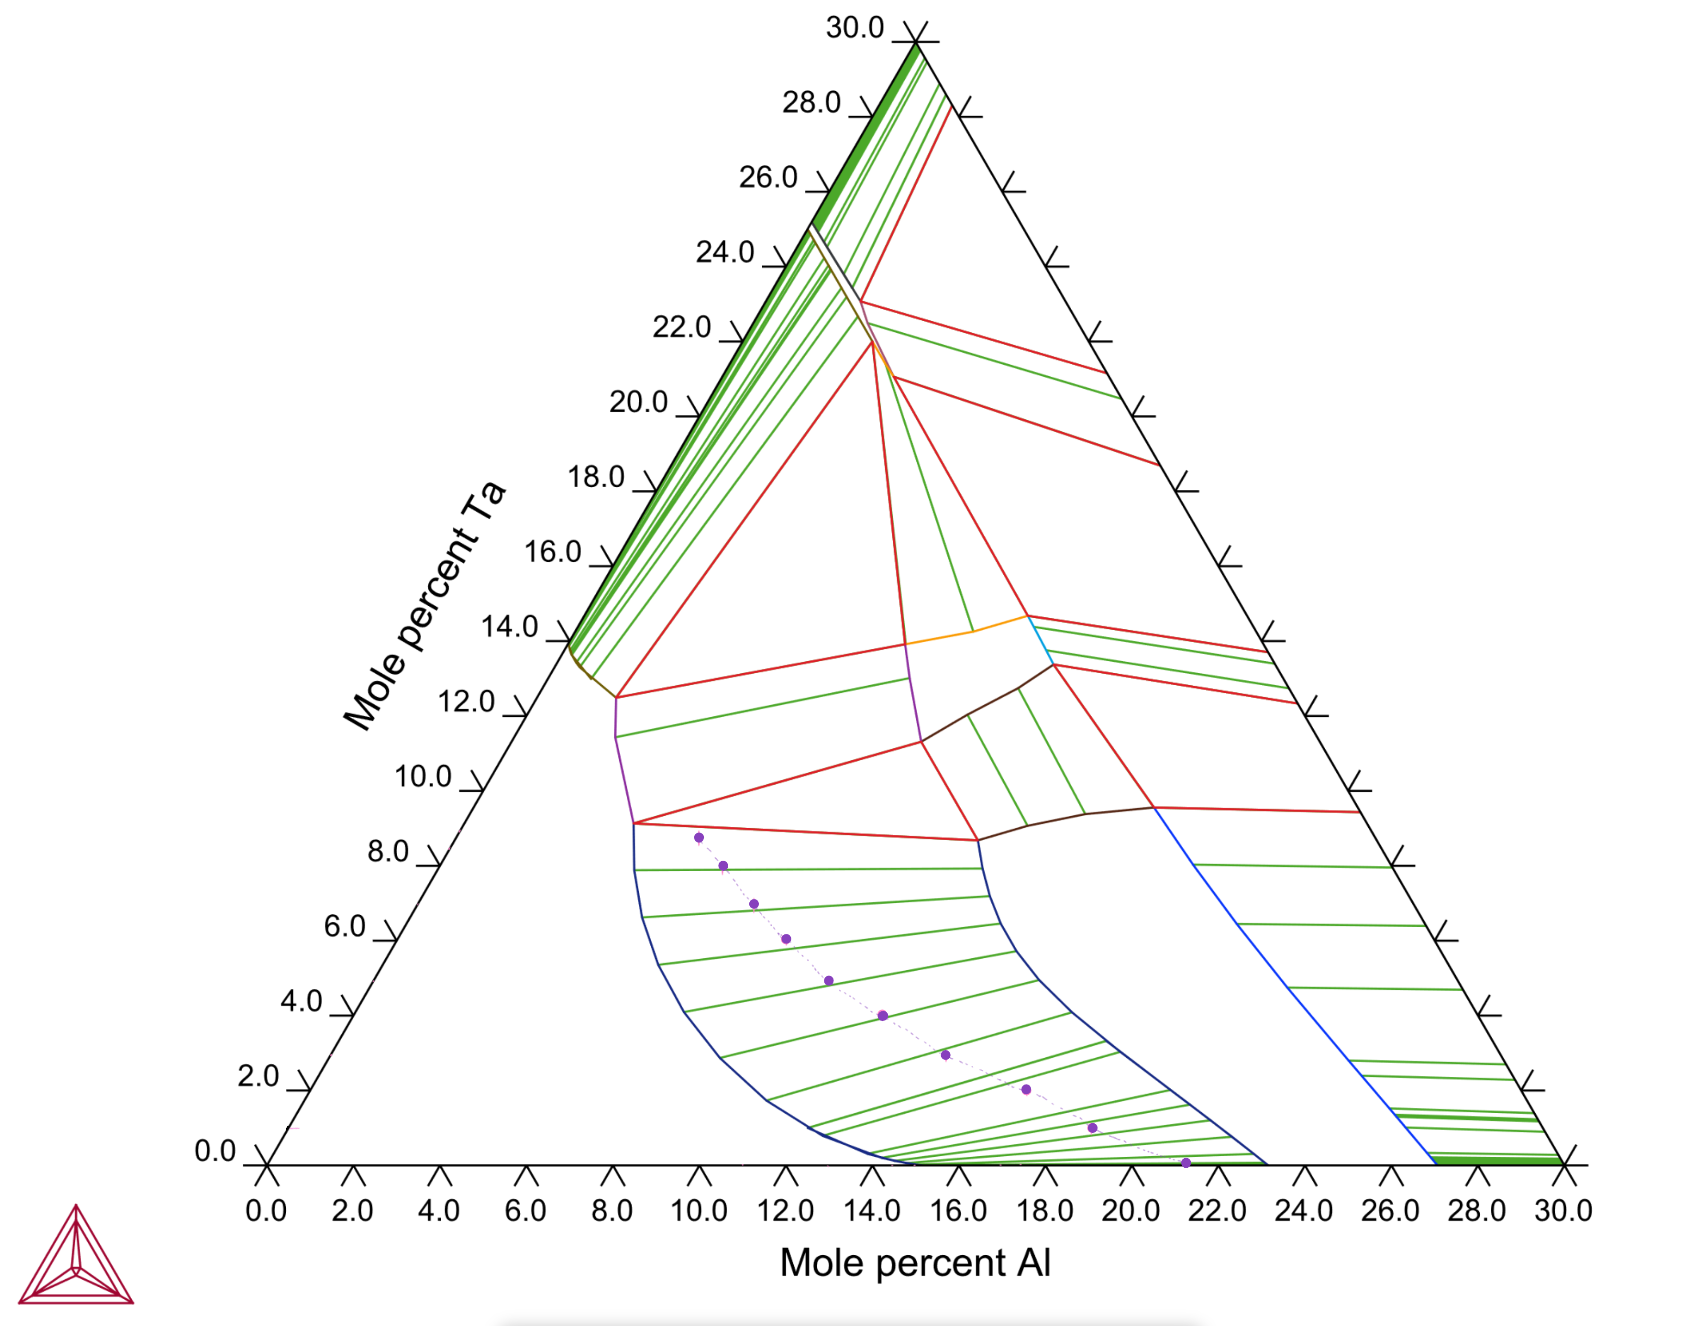
\includegraphics[width=0.95\textwidth]{graficas/Q2_NiAlTa_ternary03.png}
  \caption{Ni-Al-Ta ternary phase diagram with compositions for optimal $\gamma'$ phase fraction, $75\%$, generated using \textit{ThermoCalc} \citep{thermocalc}.}
  \label{fig:diagram03}
\end{figure}